\subsection{Architectuur}
Canvas.hs heeft een redelijk gecompliceerde architectuur. Dit komt vooral door de verschillende technologieën die nodig zijn om het HTML5 Canvas te verbinden met de te ontwikkelen Haskell API voor het bouwen van interfaces. In \autoref{fig:overzicht_architectuur} is een schematische weergave van de architectuur weergegeven.

\begin{figure}
\begin{center}
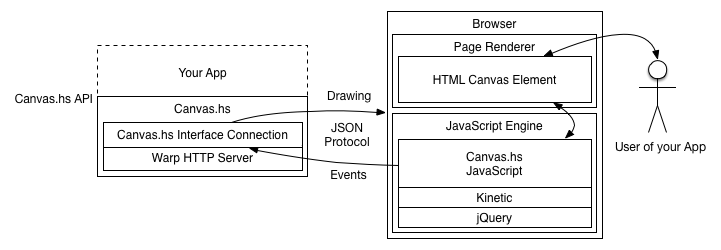
\includegraphics[keepaspectratio,width=\textwidth]{./Hoofdstukken/architecture.png}
\caption{Overzicht van de architectuur van Canvas.hs}
\label{fig:overzicht_architectuur}
\end{center}
\end{figure}

\subsubsection{Haskell}
Canvas.hs is een library die de programmeur kan importeren in zijn programma om er daarna met de API die Canvas.hs aanbiedt gemakkelijk een uitgebreide user interface mee te bouwen. Canvas.hs zal zich focussen op elementaire input en geen ondersteuning hebben voor high level interface elementen zoals buttons en textarea's. Deze elementen zouden met behulp van Canvas.hs wel eenvoudig te implementeren moeten zijn.

\paragraph{API}
De programmeur die gebruik maakt van Canvas.hs zal op een eenvoudige wijze gebruik kunnen maken van onze library. Daarom is het belangrijk dat er een API aangeboden wordt die eenvoudig te begrijpen is en niet teveel features bevat maar daarnaast wel de flexibiliteit biedt om een zeer complexe interface mee te bouwen.

\paragraph{Verbinding met de interface}
De verbinding met het canvas wordt bewerkstelligd met een eenvoudige HTTP server. Deze server biedt de gebruiker de mogelijkheid om via een webbrowser het Haskell programma te benaderen. De HTTP server biedt pagina's aan waarin JavaScript en HTML samenwerken om op het canvas te tekenen.

Als via de API van Canvas.hs begonnen wordt met tekenen zal de HTTP server automatisch gestart worden. Het besturingssysteem wordt aangeroepen voor het openen van de standaard browser --verwijzende naar het adres van de lokaal draaiende HTTP server.
\subsubsection{Protocol}
De gegevens die verstuurd worden volgens het protocol zullen op een primaire gegevensstructuur moeten aanhouden. Hiervoor kunnen twee voor de hand liggende conventies gekozen worden: XML en JSON. Ons protocol zal gegevens coderen in JSON (JavaScript Object Notation). De voordelen van JSON zijn onder andere dat de data met weinig moeite direct gebruikt kan worden in JavaScript, lichtgewicht is en makkelijk te lezen is.
\paragraph{Websockets}
Gegevensoverdracht tussen de HTTP server en de browser moet snel gebeuren zonder een al te groote vertraging. Er zijn in de communicatie tussen een HTTP server en client verschillende mogelijkheden waarbij websockets de meestvoordehand liggende is. Websockets is een relatief nieuwe feature van HTTP en wordt op dit moment alleen ondersteund in de nieuwe browsers. Het gebruik van websockets zou als gevolg hebben dat Canvas.hs geen ondersteuning heeft voor oudere browsers.
\paragraph{Restful vs RPC}
Naast de manier waarop gegevens worden gecodeerd is het ook belangrijk via welke wegen deze aan de server worden aangeboden—alsmede hoe deze door de server worden verstrekt.

RESTful HTTP webservices hebben als voordeel dat deze de basis en de functionaliteit van het HTTP protocol optimaal benutten voor het verder defineren van een eigen protocol. RPC geeft de vrijheid om een volledig, zelf in te vullen, protocol te bouwen op het HTTP protocol. Gezien de werkbaarheid van WebSockets nog onderzocht moeten worden is het de vraag welke aanpak er uiteindelijk gebruikt zal gaan worden.

Voor AJAX requests middels HTTP fetching zou een RESTful webservice een goede optie zijn. Echter is bij WebSockets het HTTP protocol niet meer beschikbaar en zal er gebruik gemaakt moeten worden van een vorm van RPC. 
\paragraph{Interface data}
De gegevens die door de HTTP server naar de browser gestuurd worden zullen voornamelijk bestaan uit interface data. Hoe, is de interface opgebouwd, elke elementen staan waar, welke attributen hebben deze elementen en zijn deze elementen in staat input van de gebruiker te accepteren. Hierbij zal er in het protocol rekening gehouden worden met de weergave van de elementen. De elementen die Kinetic.js ondersteund bieden hier een goede basis voor.
\paragraph{Events}
Events zijn de gegevens die de browser terug stuurt naar de HTTP server. Deze gegevens zullen vooral informatie bevatten over interface acties die de gebruiker uitvoerd. Het gaat hierbij om bijvoorbeeld muisbewegingen, muisklikken en toetsaanslagen. Het is belangrijk dat deze events snel door de server worden ontvangen en verwerkt naar nieuwe output zodat de gebruiker geen zichtbare vertraging ziet in de werking van het programma.

\subsubsection{Javascript}
Voor het tekenen van de interface op het HTML Canvas alsmede de communicatie vanuit de browser met de server, zal er gebruik worden gemaakt van JavaScript. jQuery biedt een prima uitbreiding op JavaScript waarbij de mogelijkheid wordt geboden verschillende zogenaamde jQuery plugins te gebruiken. In het geval van Canvas.hs zijn twee plugins belangrijk: Kinetic.js en jQuery-websockets.

Kinetic.js zal gebruikt worden voor het tekenen van de verschillende elementen op het canvas. Daarbij heeft Kinetic.js in compinatie met jQuery ook uitstekende ondersteuning voor het doorgeven van input events, die door bijvoorbeeld muisbeweginen aangeroepen worden. 

jQuery-websockets is een plugin die het gemakkelijk maakt gegevensoverdracht tussen websockets af te vangen en daar snel actie op te ondernemen. Deze lichtgewicht library maakt het mogelijk snel, zonder veel overhead opdrachten door te sturen naar Kinetic.js zodat deze op het canvas getekend worden.

\paragraph{Debug Console}
Voor de programmeur die gebruik gaat maken van de Canvas.hs library is het belangrijk dat zijn interface er zo uit ziet zoals hij dit wil. Ongetwijfeld zal een programmeur tegen problemen aanlopen bij het bouwen van de interface die hij niet had voorzien bij het schrijven van zijn code. Daarom vinden wij het belangrijk dat de interface van Canvas.hs een zogenaamde dubug console bevat waar het aanroepen van teken functies en de invloed van deze API aanroepen goed visueel en tekstueel inzichtelijk worden.
